\section{KB-Plot/Virtual Wall Rendering}

To evaluate the capability of the system to render virtual dynamics, a KB-plot is created. In our case we investigate the rendering of a virtual wall. To do so, we search for KB-pairs as large as possible with the system still being stable. In case that the wall is placed at an angle $\theta = 0$, the motor torque is calculated as follows:

\begin{equation}
    \tau = K*\Delta\theta - B*\dot{\theta}
\end{equation}

With the results, we can also measure how well the wall is rendered by measuring the created force on the user.

\subsection{Implementation}

As mentioned before, we want to find KB-pairs with a stable wall rendering. The program is simple, one can set the values for K, B and the wall position manually. After starting the simulation, the tester has to move the end-effector into the wall with his/her own hand. One can then move it around a little to test if one can find any instability. Even if a small instability is found, the values have to be reduced!

\textbf{Attention!} The program only generates counter-clockwise torques and the wall always goes from you angle to clockwise direction. Therefore you have to make sure that the end-effector is on the left side of the wall when you start the simulation.

In the program one can also choose the velocity estimation method. There are three possibilities: 

\begin{enumerate}
    \item Tacho (standard)
    \item Encoder Derivation (Finite Differentiation Method (FDM))
    \item First Order Adaptive Windowing (FOAW) with window size of 20 samples and d=0.05
\end{enumerate}

They should all be used once in order to compare the different methods.

After the measurement for the KB-Plot is done, one can apply the maximum KB-pair found and measure the force in the force sensor by pushing the end-effector into the wall. 


\subsection{Data Analysis}

In this case the data analysis is very simple. No data has to be recorded, since the stable KB-pairs have to be determined manually. The KB-pairs have to be written to a separate excel file, with which they can be read into python and can then be plotted.

For the virtual wall rendering we have to measure the force (force sensor) as well as the position. We can then plot the force over the the position in order to evaluate the rendering.

\subsection{Results}

In the following the results are presented. There is always one curve for FDM, tacho and FOAW respectively. As is visible, the results are similar. However, the values are smaller than the ones in Monika's ICORR paper ($K_{max} = 1.3\frac{Nm}{deg}, B_{max} = 0.0012\frac{Nm*s}{deg}$). This could be because the test is not very objective and a lot depends on the feeling of the testing person.

The measured values for MIKE \#3 and MIKE \#6 are comparable to each other. We can see that using the tacho generates the highest possible values for K, while FDM allows for the largest damping.

\begin{figure}[h]
    \begin{minipage}[m]{0.5\textwidth}
     \centering
        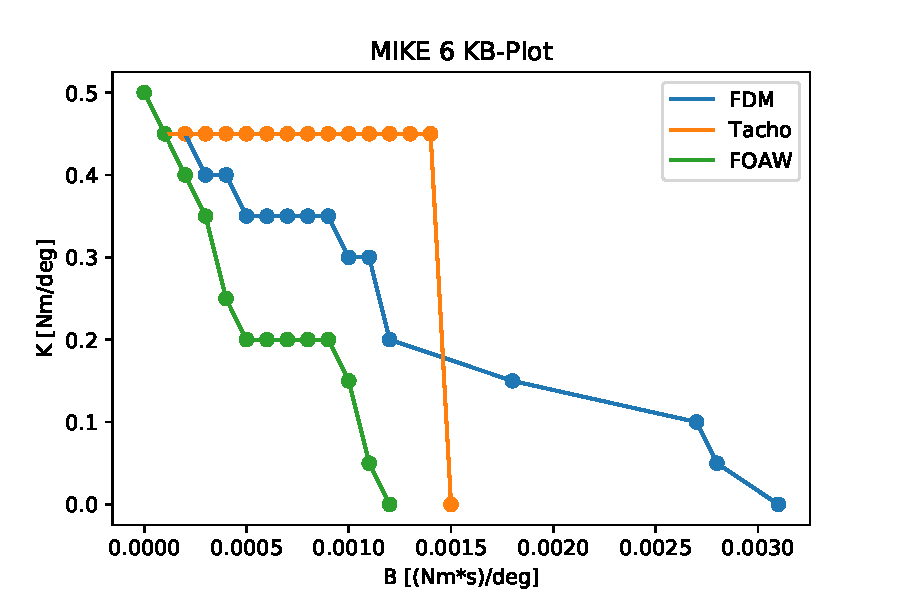
\includegraphics[width = \textwidth]{chapters/kb_plot/Mike6_KB_Plot.pdf}
    \end{minipage}
    \hfill
    \begin{minipage}[m]{0.5\textwidth}
     \centering
        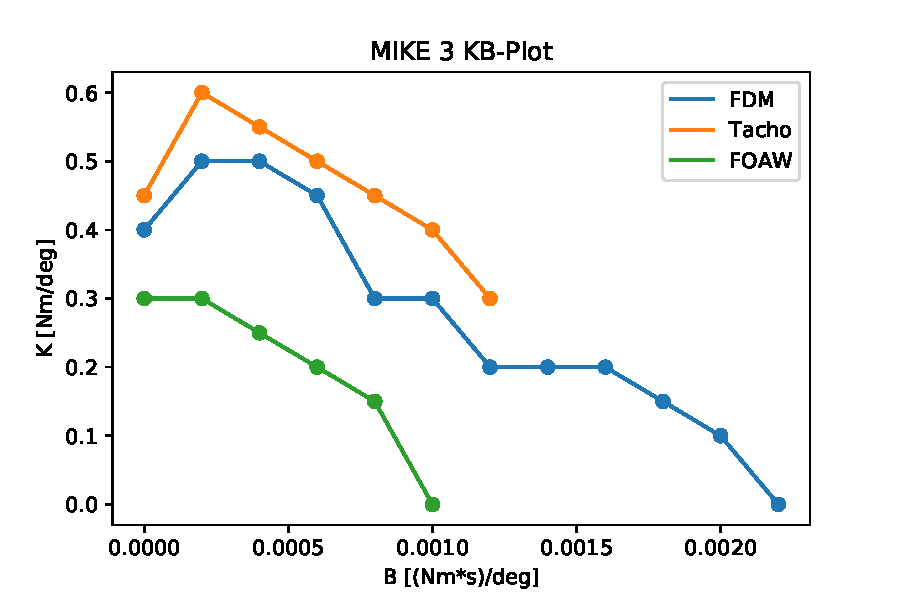
\includegraphics[width = \textwidth]{chapters/kb_plot/Mike3_KB_Plot.pdf}
    \end{minipage}
    \caption{KB-plots of MIKE \#6 and MIKE \#3.}
\end{figure}

\clearpage
In the following the force exerted by the wall is visualized. MIKE \#3 generates higher forces since its motor can generate more torque. However, if pushed too much, MIKE \#3 will collapse and cannot hold the maximum force while MIKE \#6 can continuously hold its maximum force. This can either be because of hardware or because of a safety feature implemented in the software, I am not sure about that. As in this test, the end-effector was moved by hand, the influence of B (damping) is small, because the velocity is low. Therefore, the important parameter is K (stiffness). 

\begin{figure}[h]
    \begin{minipage}[m]{0.5\textwidth}
     \centering
        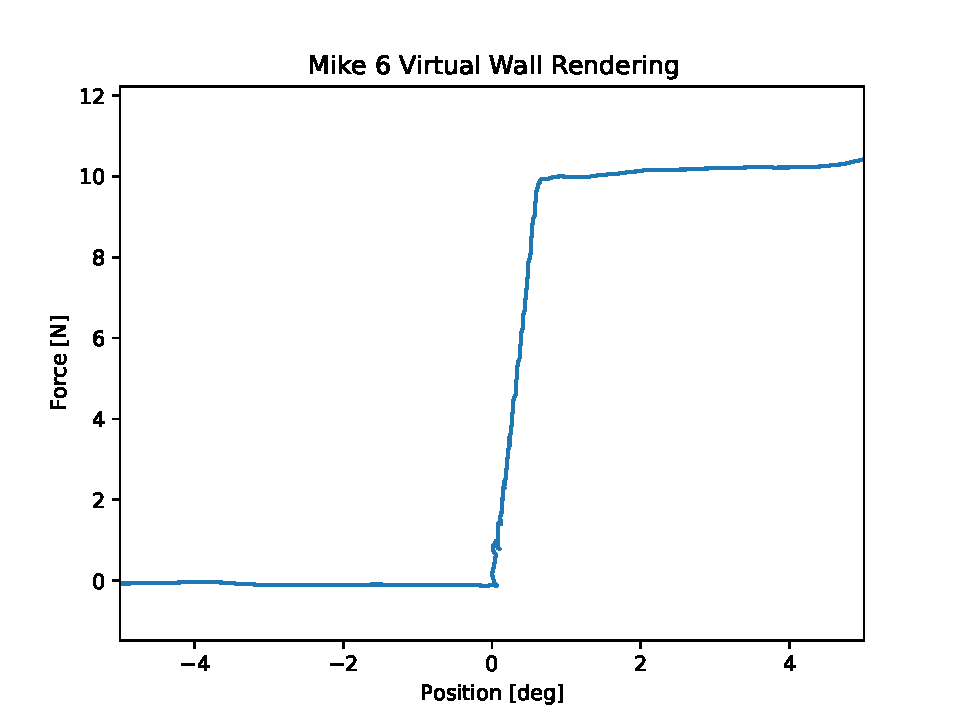
\includegraphics[width = \textwidth]{chapters/kb_plot/Mike6_VirtualWall.pdf}
    \end{minipage}
    \hfill
    \begin{minipage}[m]{0.5\textwidth}
     \centering
        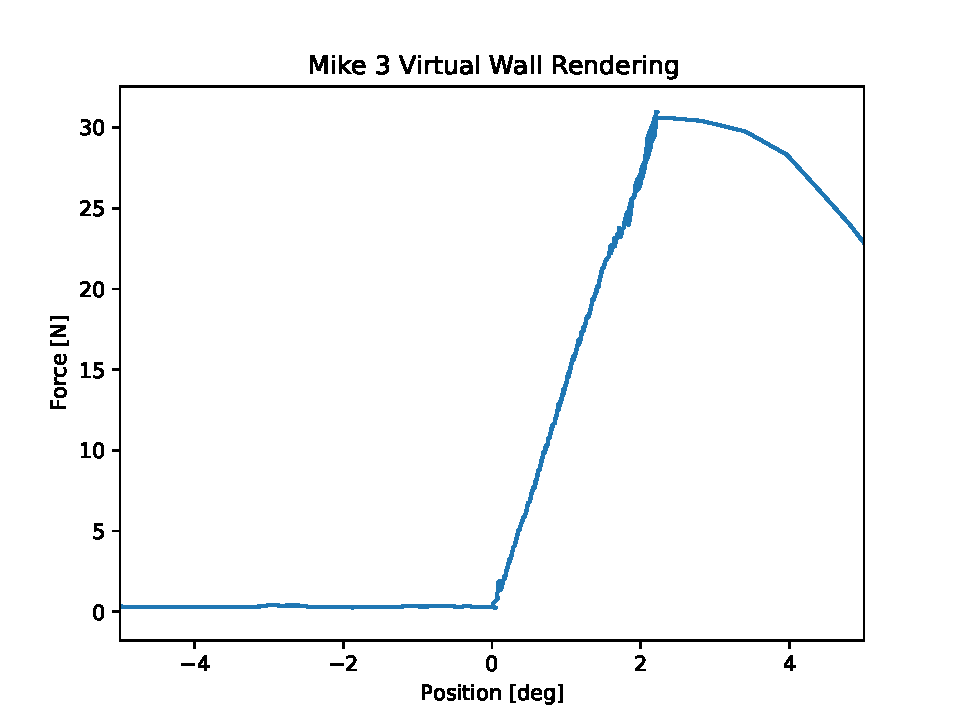
\includegraphics[width = \textwidth]{chapters/kb_plot/Mike3_VirtualWall.pdf}
    \end{minipage}
    \caption{Left: MIKE \#6, with K=0.45 and B=0.0014; Right: MIKE \#3, with K=0.6 and B=0.0003}
\end{figure}